\section{Mathematical Basic}
\subsection*{Identities and Inequalities}
Binomial expansion theorem:\\
$(x+y)^n=\sum_{i=0}^{n}\binom{n}{i}x^i y^{n-i}$\\
Proposition:\\
\begin{itemize}
    \item For all $x\ge 1$ it holds that $(1-1/x)^x\le e^{-1}$
    \item For all $x$ it holds that $1-x\le e^{-x}$
    \item For all $x$ with $0\le x \le 1$ it holds that
\end{itemize}
$e^{-x}\le 1-(1-\frac{1}{e})\cdot x\le 1-\frac{x}{2}$\\
\subsection*{Asymptotic Notation}
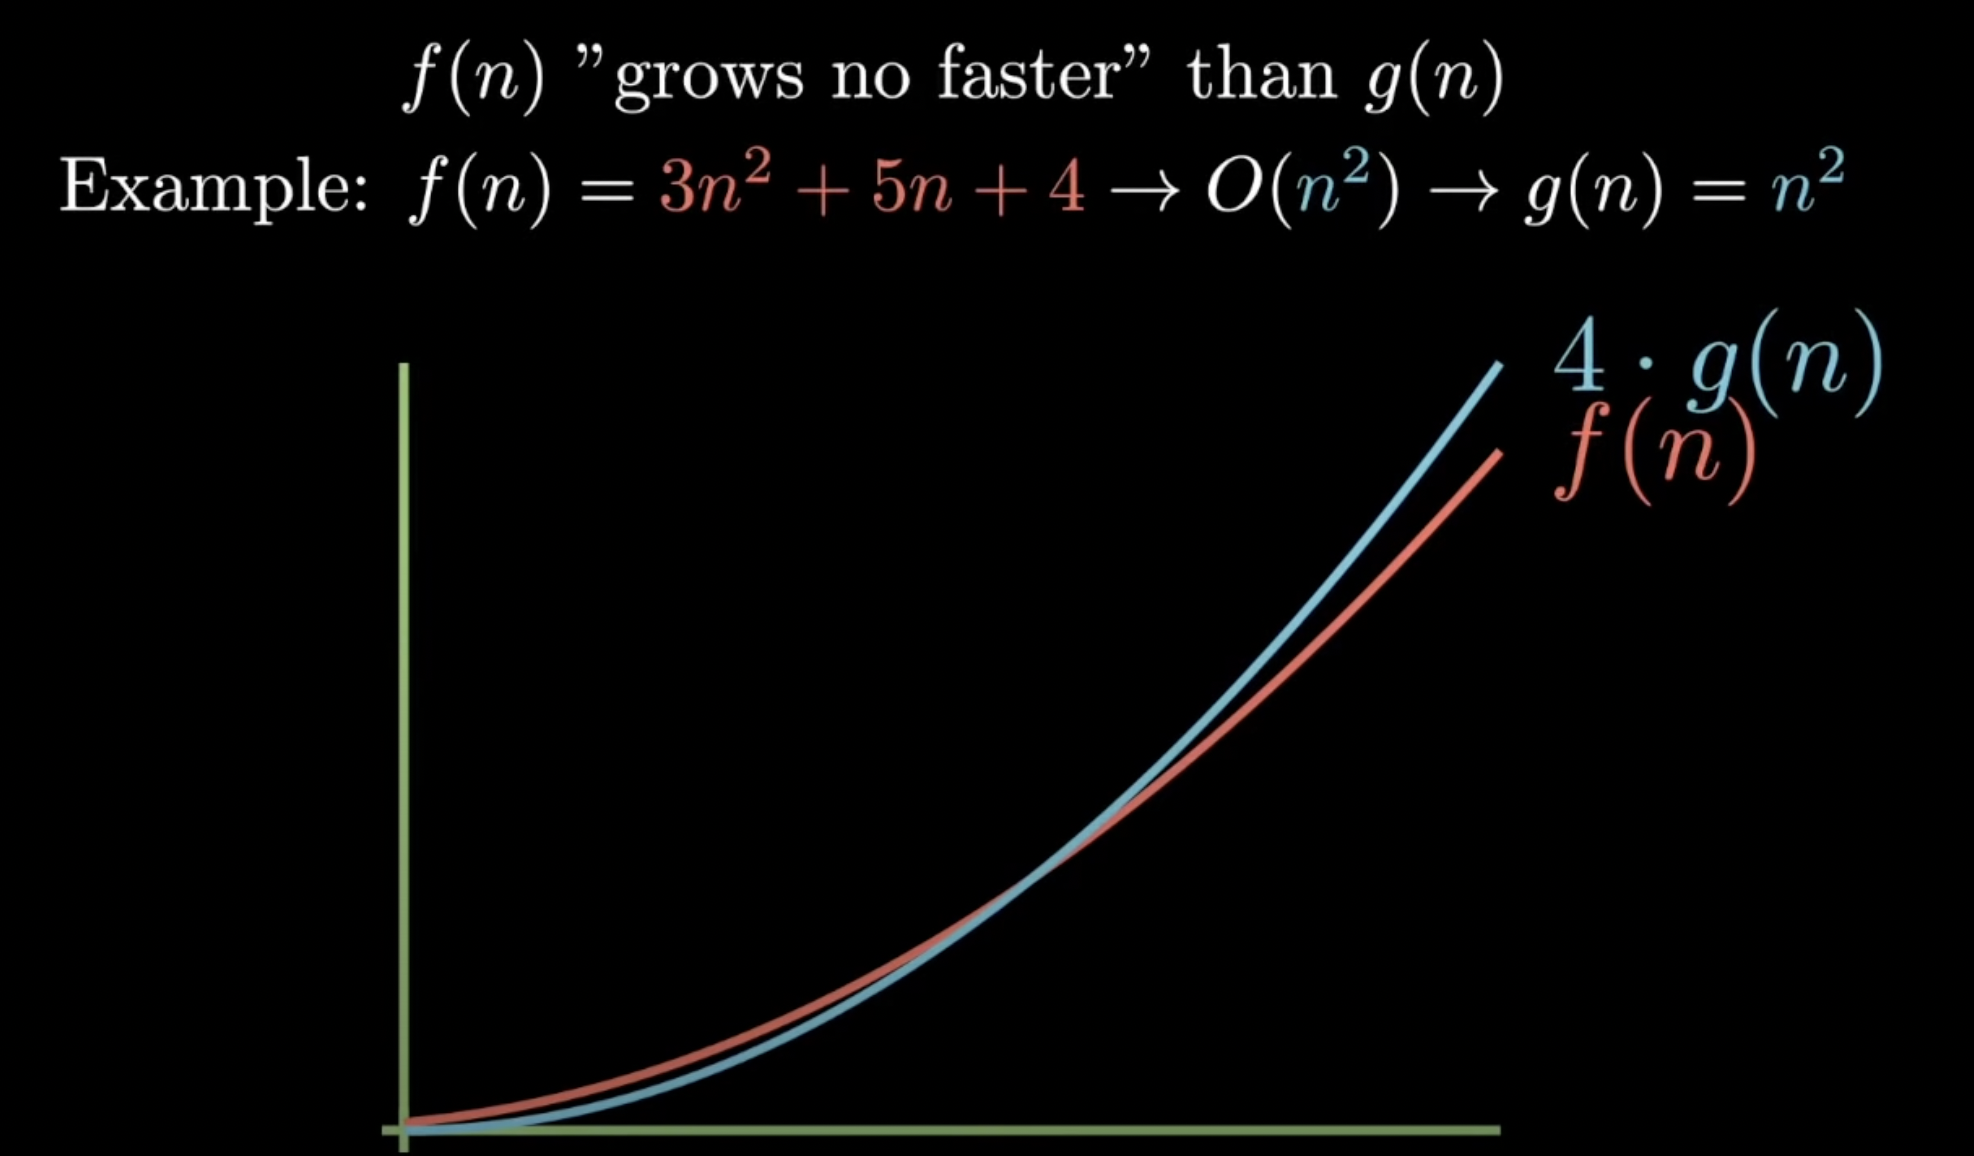
\includegraphics[width=\columnwidth]{big-o-explained.png}
Let $f(n),g(n)$ be functions from non-negative integers to non-negative reals. 
Then:
\begin{itemize}
    \item $f(n)=\mathcal{O}(g(n))$ means that there exist positive integers c 
    and n' such that for all $n > n'$ it holds that $f(n)\le c \cdot g(n)$
    \item $f(n)=\varOmega (g(n))$ means that there exist positive integers c
    and n' such that for all $n > n'$ it holds that $f(n)\ge c\cdot g(n)$.
    \item $f(n)=\varTheta (g(n))$ means that there exist positive integers 
    $c_{1}$ and $c_{2}$ such that for all $n > n'$ it holds that 
    $c_{1}\cdot g(n) \le f(n) \le c_{2} \cdot g(n)$
    \item $f(n)=o(g(n))$ means that $\lim_{n \to \infty} \frac{f(n)}{g(n)}=0$ 
    \item $f(n)=\omega (g(n))$ means that 
    $\lim_{n \to \infty} \frac{f(n)}{g(n)}=\infty$ 
\end{itemize}

\subsection*{Basic Probability}

By definition:\\
$\Pr[E] = 1 - \Pr[\bar{E}]$\\
$\Pr[E_1\wedge E_2]\le \Pr[E_1]$\\
$\Pr[E_1 \vee E_2]\ge\Pr[E_1]$\\
When $E_1$ $E_2$ are independent:\\
$\Pr[E_1\wedge E_2]=\Pr[E_1] \cdot \Pr[E_2]$\\
Union Bound:\\
$\Pr[E_1\vee E_2]\le\Pr[E_1]+\Pr[E_2]$\\
Bayes' Theorem:\\
$\Pr[E_1|E_2] = \frac{\Pr[E_2|E_1]\cdot\Pr[E_1]}{\Pr[E_2]}$\\
Let $E_1,\cdots ,E_n$ be events such that $Pr[E_1\vee\cdots E_n]=1$ and 
$\Pr[E_i\wedge E_j]=0$ for all $i\neq j$. That is, the ${E_i}$ \emph{partition} 
the space of all possible events, so that with probability 1 exactly one of the
events $E_i$ occurs. Then for any F:\\
$\Pr[F]=\sum_{i=1}^{n}\Pr[F\wedge E_i]$\\
when $n=2$ and $E_2=\bar{E}_1$, giving:\\
$\Pr[F]=\Pr[F|E_1]\cdot\Pr[E_1]+\Pr[F|\bar{E}_1]\cdot\Pr[\bar{E}_1]$\\
we get a tighter union bound:\\
$\Pr[E_1\vee E_2]\le\Pr[E_1]+\Pr[E_2|\bar{E}_1]$\\
$\Pr[\vee^{k}_{i=1}E_{i}]
\le\Pr[E_1]+\sum^{k}_{i=2}\Pr[E_i|\bar{E}_1\wedge\cdots\wedge\bar{E}_{i-1}]$\\